\title{Manual de uso del editor de texto \texttt{Vim}}
\author{Gabriel López}
\date{\today}

\documentclass[10pt]{article}
\usepackage[spanish]{babel}
\usepackage{graphicx}
\usepackage[letterpaper]{geometry}
\usepackage{lmodern,minted}
\usepackage{blindtext}
\usepackage{hyperref}
\usepackage{forest}


\begin{document}
\maketitle

\section{\texttt{Vim}, un editor de texto minimalista.}
\texttt{Vim} es un editor de texto creado por Brian Moolenaar. Es una versión mejorada del editor de texto \texttt{vi} creado por el programador Bill Joy. 
El editor de texto \texttt{Vim} es un editor de texto pensando para ser un programa de edición de texto minimalista y extensible, lo que significa que con ayuda de programas auxiliares hechos por la comunidad conocidos como \textit{plugins}, se puede utilizar el editor \texttt{Vim} como un entorno de programación (conocido como \textit{IDE}) o un entorno minimalista de edición de documentos hechos en \LaTeX. \\ 
Si bien, aprender a usar \texttt{Vim} es un proyecto con un curva de aprendizaje un poco pronunciada, este editor ofrece ciertas ventajas por sobre otros editores, sobre todo a nivel de personalización, configuración y uso de recursos, lo que lo hace ídoneo en \textit{hardware} de capacidad limitada. 
Además de esto, con la correcta configuración y el correcto uso de \textit{plugins}, la escritura (sobre todo de documentos de tipo científico) puede ser más fluida a un nivel muy similar a la toma de notas manuscritas. 
\section{Entornos en \texttt{Vim}}
\texttt{Vim} es un editor de texto poco ortodoxo comparado con el resto de los editores de texto que están disponibles para uso público, para empezar, \texttt{Vim} usa un esquema de entornos \textit{entornos}, lo que quiere decir, que para las acciones que usualmente se ven relegadas al uso del ratón en otros editores, en \texttt{Vim} están relegadas a un \textit{entorno}. Los entornos de uso básico son los siguientes:
\begin{itemize}
	\item \textit{NORMAL}: Este entorno es el entorno básico de \texttt{Vim}. En este entorno se utiliza para navegar entre líneas de texto, borrar contenido y introducir comandos dentro del editor.
	      La utilidad del modo \textit{NORMAL} radica en el uso de comandos para usar la terminal y el editor al mismo tiempo. 
	\item \textit{INSERTAR}: Este entorno se utiliza para la inserción de texto dentro de líneas en el editor. Para entrar a este entonro basta con introducir la tecla \texttt{i} mediante el teclado.
Una vez que la tecla se ha introducido, el editor colocará el texto \texttt{INSERTAR} o \texttt{INSERT} en la parte inferior de la pantalla, denoatando que el modo de inserción está activado. 
	\item \textit{VISUAL}: Este entorno se encarga de función de copiar y pegar contenido de las lineas. Para entrar a este modo, se debe introducir \texttt{v} con el teclado.
Una vez que el modo \textit{VISUAL} está activado debe aparecer en pantalla la leyenda \texttt{VISUAL} en la esquina inferior izquierda. 
\end{itemize}
Es importante destacar que para salir de un entorno para entrar de nuevo al entorno \textit{NORMAL} se introduce la tecla \texttt{Esc} con el teclado. Para ilustrar los entornos de \texttt{Vim} colocamos la siguiente imagen. En dicha imagen es notorio que debido al idioma con el que se tiene el ordenador, aparece la leyenda \texttt{INSERTAR} en la parte inferior, denotando que el modo de inserción de texto está activo. 
\begin{figure}[h]
	\centering
	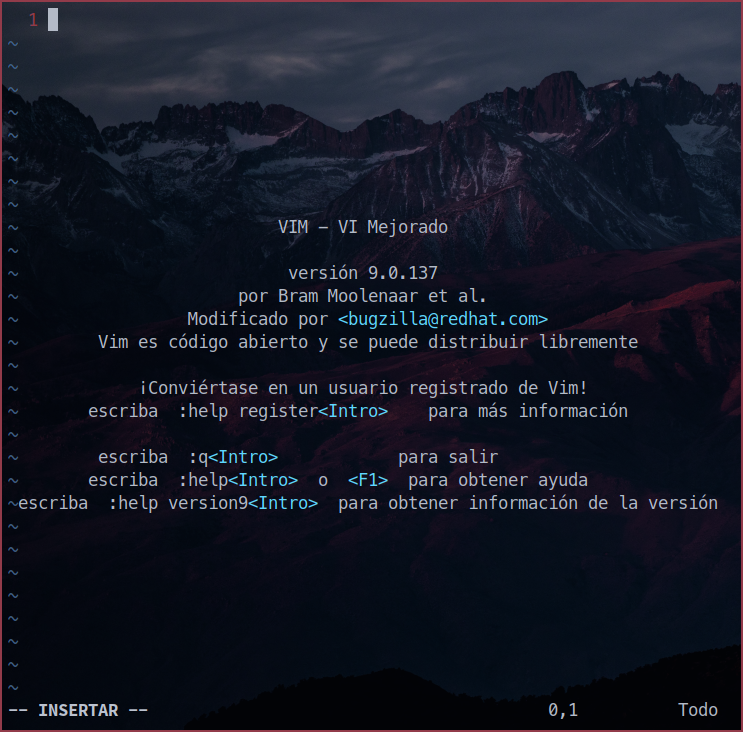
\includegraphics[scale=0.6]{./img/Vim_INS.png}
	\caption{\texttt{Vim} en el modo \textit{INSERTAR}}
\end{figure}
\newline
A pesar de todo esto, existen muchos más entornos dentro del editor, sin embargo, consideramos que estos tres son los más útiles para un usuario nuevo de \texttt{Vim} debido a que facilitan la escritura de documentos y permiten la introducción de comandos dentro del mismo. 
\newpage
\section{¿Cómo salir de \texttt{Vim}?}
Es normal que el usuario novato de GNU-Linux o cualquier sistema operativo derivado de UNIX. De modo que el sistema operativo a veces deja el usuario dentro de \texttt{Vim} sin ningún aviso de cómo salir del editor de texto. Por esta razón en esta sección se explicará como salir de \texttt{Vim}. \\
Para empezar, la imagen inicial que el usuario tiene al entrar a \texttt{Vim} es la siguiente: \newline
\begin{figure}[h]
	\centering
	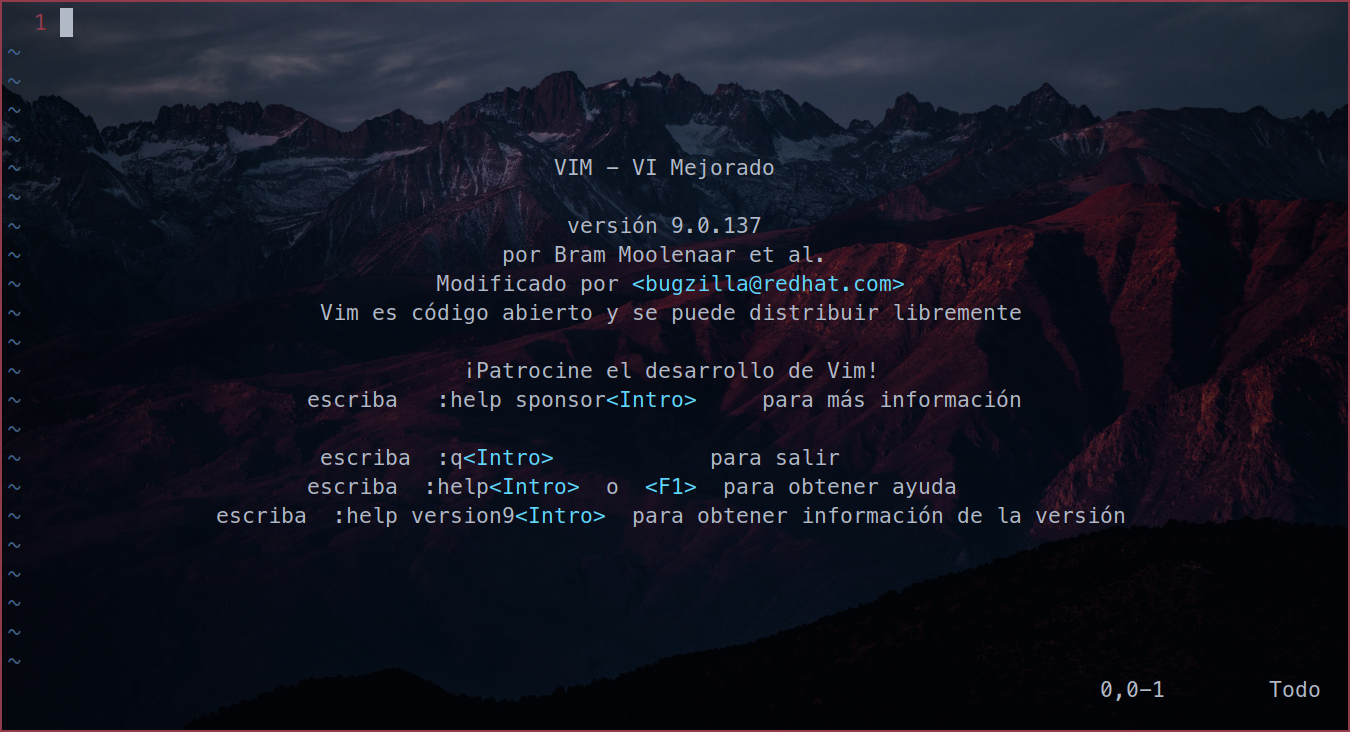
\includegraphics[scale=0.4]{./img/poisson_mu1.png}
	\caption{Primera impresión de \texttt{Vim}}
\end{figure}
\newline
Podría parecer que \texttt{Vim} es complicado, pero en realidad, salir del editor es relativamente sencillo, la secuencia de pasos para salir de \texttt{Vim} es la siguiente:
\begin{itemize}
	\item Primero, si usted desea guardar el contenido del archivo, es conveniente guardar el contenido del archivo primero, esto se logra mediante el comando \texttt{:w} dentro del entorno \textit{NORMAL}.
	\item Ahora que el archivo está guardado, es posible salir del editor sin problemas, por lo que se procede a colocar el comando \texttt{:q} dentro del mismo entorno \textit{NORMAL}.
\end{itemize}
Si bien es posible que queramos guardar el contenido de nuestro archivo de texto, también tenemos la opción de salir sin guardar (no recomendada a menos que se desee salir de \texttt{Vim} si se entró por error), en este caso, basta con introducir el comando \texttt{:q!} en el modo \textit{NORMAL} del editor.
\section{¿Existe alguna forma de aprender \texttt{Vim} mediante ejemplos?}
Si bien \texttt{Vim} es un editor de texto que puede parecer poco ortodoxo al principio, existen formas para aprender su uso de una forma interactiva mediante ejemplos. En el caso de \texttt{Vim} existe el complemento denominado \texttt{vimtutor}, que es un complemento de consola que suele estar instalado en cualquier máquina UNIX. En el caso de querer acceder a dicho complemento, basta con introducir el comando \texttt{vimtutor} dentro de la terminal de GNU-Linux o su equivalente en UNIX. 
\section{Navegación en \texttt{Vim}}
\texttt{Vim} es un editor de texto que tiene un esquema de navegación diferente al resto de editores de texto que podemos encontrar en el mercado. Esto es debido a cuestiones de convención. 
Si bien, las teclas direccionales del teclado funcionan para navegar entre texto dentro del editor, su uso no es recomendado por la mayoría de guias de uso de \texttt{Vim}. 
\subsection{Navegación básica en \texttt{Vim}}
Esto se entiende mejor con los ejemplos proporcionados por el complemento de consola llamado \texttt{vimtutor}. Para nuestros efectos, se busca introducir al usuario a los conceptos básicos de los que \texttt{Vim} para que sea capaz de redactar documentos simples dentro del editor. Dicho esto, podemos mostrar el esquema básico de navegación del que hace uso \texttt{Vim}.
\begin{figure}[h]
	\centering
	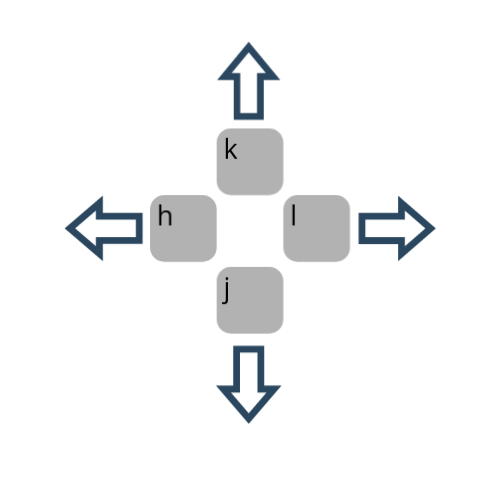
\includegraphics[scale=0.3]{./img/vim_nav.png}
	\caption{Esquema de navegación básico dentro de \texttt{Vim}}
\end{figure}
\newline
Para resumir, podemos ver que las teclas de navegación son las siguientes:
\begin{itemize}
	\item \texttt{k} y \texttt{j} son usadas para subir y bajar de linea, respectivamente. 
	\item \texttt{h} y \texttt{l} son usadas para desplazarse de izquierda a derecha, respectivamente. 
\end{itemize}
Como se puede ver, el esquema de navegación dista de los editores convencionales. Esto es por diseño, ya que  \texttt{Vim} hace uso de estas mecánicas de movimiento para tratar dicho movimiento como si fuera un \textit{comando de consola} y esto permite aplicar ciertos comandos, como el de \textit{borrar} al movimiento para alcanzar cierta velocidad a la hora de borrar contenido dentro de una línea de texto. 
\newpage
\subsection{Otras opciones de movimiento en \texttt{Vim}}
Como se mencionó anteriormente, \texttt{Vim} trata el movimiento como si fuera un comando de consola, esto permite aplicar ciertos efectos al movimiento.
Si bien, el movimiento básico se resume con las teclas, \texttt{h,j,k} y \texttt{l}, existen también cuatro comandos útiles que deben ser mostrados para que este manual se pueda considerar una referencia útil para el uso de \texttt{Vim}.
En general, \texttt{Vim} suele trabajar por \textit{palabras}cuando se habla de navegación dentro de una linea de texto, entonces existen formas para desplazarse en una linea de texto de palabra en palabra. En este caso, existen cuatro comandos destinados para esta función:
\begin{itemize}
	\item El comando \texttt{w} permite al usuario desplazarse desde su localización actual hacia el \textit{inicio} de la siguiente palabra en la linea de texto. 
	\item El comando \texttt{e} permite al usuario desplazarse desde su actual ubicación, hacia el \textit{final} de la siguiente palabra en la linea actual de texto.
	\item Se usa el número \texttt{0} para desplazarse hacia el \textit{inicio} de la linea.
	\item Finalmente, el comando \texttt{\$} se usa para desplazarse hacia el \textit{final} de la linea.
\end{itemize}
\section{La función de \textit{Borrar} en \texttt{Vim}}
Como cualquier editor de texto plano, usualmente queremos editar el contenido de nuestro archivo, ya sea cambiando algunas lineas dentro del archivo o \textit{borrando} contenido dentro de las líneas. En \texttt{Vim} la función de \textit{borrar} dentro del documento está relativamente ligada al uso de movimiento.\\
Esto es debido a que podemos pensar en lo siguiente: la función de borrar se activa con el comando \texttt{d} y la cantidad de contenido a borrar se determina usando los comandos de movimiento vistos anteriormente. Por lo que, para ilustrar algunos de los usos de este mecánica, es conveniente colocar algunos de los comandos más utilizados con esta modalidad. 
\begin{itemize}
	\item El comando \texttt{dw} permite borrar todo lo que está desde \textit{la ubicación actual hasta el inicio de la siguiente palabra.} Como ven, el comando de \textit{borrar} se antepone a la opción de movimiento.
	\item Introduciendo \texttt{de} podemos borrar todo aquello que está comprendido desde \textit{la localización del puntero en el editor, hasta el final de la siguiente palabra en la linea}. 
\end{itemize}
Como podemos observar, el comando de \textit{borrar} en \texttt{Vim} usualmente está antes de la opción de movimiento. Sin embargo, debido a razones que los creadores de \texttt{Vim} comentan en \texttt{vimtutor} es común que se requiera \textit{borrar una o más lineas completas}. \\
En este caso, la función de borrar es mucho más sencilla, solamente basta con introducir el comando \texttt{dd}. Es en este punto en donde es conveniente introducir una figura que está presente también en \texttt{Vim} y que al día de hoy, no hemos visto en otros editores de texto y que, al día de hoy, no hemos visto en otros editores de texto, esta característica se conoce como \textit{contadores}.
\subsection{Contadores}
Los \textit{contadores} son una característica de \texttt{Vim} que permite al usuario repetir un comando un determinado número de veces, usualmente \texttt{vimtutor} relega la lección de esta característica hasta que ya se han visto los comandos básicos de movimiento y borrado y en este caso, es conveniente explicar un poco el porqué. Supongamos lo siguiente: Se desea borrar un número determinado de líneas en el editor, si se usaran otros editores, se podría pensar en usar el ratón para seleccionar las líneas y borrarlas con la tecla \texttt{backspace}.\\
Sin embargo, en \texttt{Vim} se debe aplicar el uso de los comandos vistos anteriormente. Un ejemplo simple sería el borrado de 4 lineas en un archivo de texto. En este caso, el comando a utilizar es: \texttt{4dd}. La explicación del comando es la siguiente: 
\begin{itemize}
	\item \texttt{4} es el número de veces que se repetirá el siguiente comando. 
	\item \texttt{dd} es el comando usado para borrar una linea completa en el documento de texto. 
\end{itemize}
Este es el uso más sencillo de los contadores en \texttt{Vim}, sin embargo, su uso no se limita solamente a esto, y es recomandable revisar la sección de contadores en el complemento \texttt{vimtutor} para una mejor comprensión del uso de esta característica del editor.
\section{Configuración del archivo \texttt{.vimrc}}
\texttt{Vim} es un programa de UNIX, lo que significa que como una gran mayoría de los programas de terminal que se usan en esta plataforma, este usa un archivo de configuración. Este archivo se encuentra en el directorio \texttt{\$HOME} de la terminal de GNU-LINUX, con el nombre de \texttt{.vimrc}. 
Como se puede observar \texttt{.vimrc} es un archivo oculto, por lo que es necesario cambiar las opciones por defecto en su gestor de archivos o introducir el comando \texttt{ls -a} en la terminal. \\
El archivo \texttt{.vimrc} es util para configurar opciones globales de \texttt{Vim}, estas sobre todo se refieren a \textit{qué} hacer con ciertos archivos, sobre todo a aquellos que tienen un tipo de extensión particular como ser \texttt{.tex, .c, .py}, etc. Sobre todo, \texttt{Vim} facilita ciertas cosas útiles para el usuario al momento de editar estos archivos, como ser: 
\begin{itemize}
	\item \textit{Syntax-highlighting}:  que es básicamente colocar colores a ciertas expresiones para diferenciar entre comandos y texto plano. Esto es particularmente útil con archivos de \LaTeX, dado que permite una mejora en la legibilidad del archivo.
	\item \textit{Numeración de las líneas}: como en los editores de texto modernos, \texttt{Vim} tiene la opción de asignar números a las líneas de texto. Esto facilita el \textit{depuración} del código independientemente del lenguaje de programación, porque permite revisar la línea que tiene errores dentro del archivo de reporte de errores. 
	\item \textit{Instalación de Plugins}: \texttt{Vim} permite configurar el editor para mejorar ciertas funcionalidades referentes a ciertos archivos de texto. Los plugins que serán usados en este manual son referentes a la integración de \LaTeX \ con \texttt{Vim}. Para la instalación de estos plugins, se suele incluir una línea dentro del \texttt{.vimrc} para indicar qué plugin se procede a instalar.  
\end{itemize}
Para mostrar algunas de las posibles configuraciones que pueden hacerse en el archivo \texttt{.vimrc} sin hacer instalaciones avanzadas (eso será tratado en un momento posterior en este manual) se pasa a mostrar una configuración básica del archivo \texttt{.vimrc}. 
Esta es la configuración que el autor de este documento usa hasta el momento, sin embargo, es necesario que se comprenda que muchas de las lineas que aparecen en este documento están relacionadas a los \textit{plugins} que el autor del documento mostrará más adelante.
\newpage
\subsection{Configuración básica de un archivo \texttt{.vimrc}}
\begin{minted}[linenos]{vim}
"Esto es un comentario en el archivo .vimrc"

"El siguiente comando es para colocar numero de línea al lado del editor"
:set number 
"Comando para hacer ajuste del texto al ancho de ventana"
:set wrap
"Comando usado para la instalación de plugins"
call plug#begin('~/.vim/plugged')

"INSTALACION DE PLUGINS"
"Se instalan multiples plugins con el comando Plug #nombre
"seguido del caracter |"
Plug 'SirVer/ultisnips' | Plug 'honza/vim-snippets'
Plug 'xuhdev/vim-latex-live-preview', { 'for': 'tex' }
Plug 'lervag/vimtex'
"Mas adelante se aprenderá para qué sirven los comandos situados"
"Despues del :set wrap"
\end{minted}
Como podemos ver, en realidad, las posibilidades de configurar el archivo \texttt{.vimrc} son infinitas, sobre todo porque ocultamos (por brevedad) el resto de la configuración de \textit{plugins} que se hacen dentro del archivo mencionado.
Considerando esto, podemos ver que el archivo \texttt{.vimrc} es un archivo fundamental para poder configurar a \texttt{Vim} para poder realizar tareas productivas tanto como un \textit{IDE} (para programación) o como editor de documentos de \LaTeX.
Hay que destacar que la configuración anterior es una configuración sumamente básica, es común que los usuarios avanzados de \texttt{Vim} tengan archivos de configuración de más de cien líneas. 
\section{Instalación de \textit{Plugins}}
\texttt{Vim} es un editor de texto muy básico, pero su principal ventaja es su capacidad de ser \textit{extensible} lo que permite agregar funciones a \texttt{Vim} que pueden ser:
\begin{enumerate}
	\item \textit{Syntax Highlighting} para los distintos lenguajes de programación que se usen para desarrollo de software en \texttt{Vim}.
	\item Configuración de atajos de teclado \textit{para cada uno de los lenguajes de programación usados en} \texttt{Vim}, un buen ejemplo de esto puede ser el que, si tomamos a \LaTeX \  como un ejemplo, es muy común tener que escribir \texttt{"begin"} para colocar un entorno como \texttt{equation} o \texttt{align}. Por lo que es posible configurar un atajo de teclado para evitar la escritura completa de este comando.  
\end{enumerate}
Los \textit{Plugins} en \texttt{Vim} se pueden instalar de dos formas: manual y utilizando un \textit{plugin-manager}. Debido a cuestiones más prácticas, vamos a centrarnos en la última forma de instalar los \textit{plugins}. En este caso, consideramos que es más conveniente revisar la documentación del \textit{plugin-manager} que el autor de este manual recomienda, en este caso, se recomienda empezar usando el \textit{manager} conocido como \textbf{Vim-Plug}.\\
\textbf{Comentario: Como muchas de las instrucciones de instalación de software en Linux suelen cambiar con el tiempo, consideramos más conveniente que el lector revise las instalaciones de instalación de Vim-Plug en el repositorio de GitHub de este componente software.} El repositorio de \textbf{Vim-Plug} se encuentra en la siguiente dirección web. 
\begin{center}
\url{https://github.com/junegunn/vim-plug}	
\end{center}
Una vez que se ha instalado el gestor de plugins \textit{Vim-Plug}, es posible que si requiere instalar plugins de utilidad para este manual, usted requiera cambiar algunas cosas en el archivo \texttt{.vimrc}. Los plugins de interés que el autor usa en este manual se encuentran en la subsección 7.1 de este manual. Mostramos aquí cómo es el proceso de instalación de los plugins que el autor de este manual usó para la creación de este documento. 
\begin{minted}[linenos]{vim}
"Este comando es para inicializar a Vim-Plug"
call plug#begin('~/.vim/plugged')
"Aquí le damos a Vim-Plug una lista de plugins a instalar"

"PLUGIN DE ATAJOS DE TECLADO PARA LaTeX"
Plug 'SirVer/ultisnips' | Plug 'honza/vim-snippets'

"PLUGIN PARA COMPILAR DOCUMENTOS EN TIEMPO REAL"
Plug 'xuhdev/vim-latex-live-preview', { 'for': 'tex' }

"ESTE ULTIMO PLUGIN TIENE SU PROPIA SECCION EN EL MANUAL"
Plug 'lervag/vimtex'
\end{minted}
Una vez que tengamos lo que se mostró en la sección de código anterior, es posible instalar todos estos plugins usando el comando \texttt{:PlugInstall} en el modo \texttt{NORMAL} de \texttt{Vim}, esto considerando que se requiere de una correcta conexión a internet para poder instalar de dichos plugins. Además de esto, se le recomienda al usuario investigar por su cuenta acerca de los otros plugins que existen para otros lenguajes de programación, debido a que este manual solo se centra en aspectos básicos de \texttt{Vim} y su integración con \LaTeX. 
\section{Uso básico de \texttt{Vimtex}}	
Hemos hablado de algunos plugins que son usados para integrar el editor de \texttt{Vim} con \LaTeX. En este caso, podemos hacer uso del \textit{Plugin} conocido como \texttt{Vimtex}, que es una suite de plugins para \texttt{Vim} que está orientado a integrar a \texttt{Vim} con \LaTeX. Las instrucciones de instalación de \texttt{Vimtex} de nuevo, cambian con las constantes actualizaciones que se le hacen al software, por lo que recomendamos revisar el repositorio de GitHub para \texttt{Vimtex}.
El repositorio de GitHub de \texttt{Vimtex} se encuentra en la siguiente dirección web:
\begin{center}
	\url{https://github.com/lervag/vimtex}
\end{center}
Una vez que se instale \texttt{Vimtex} en su ordenador, consideramos que es útil explicar los siguientes comandos y carácteristicas de \texttt{Vimtex} que pueden ser de utilidad para el usuario.
\subsection{Configuración del archivo \texttt{.vimrc} orientado al uso de \texttt{Vimtex}}
Como \texttt{Vimtex} es una suite de paquetes útiles para integrar \texttt{Vim} con \LaTeX, es necesario realizar algunos cuantos cambios al archivo \texttt{.vimrc} para que el plugin de \texttt{Vimtex} esté cargado cuando se ejecuta el comando \texttt{Vim} en la terminal y se requiere editar un archivo con extensión \texttt{*.tex} en la terminal. En realidad, muchas de las instrucciones acerca del cómo se debe colocar esta configuración están en elrepositorio de \texttt{Vimtex}, sin embargo, el autor de este manual si encontró algunos inconvenientes al principio para poder integrar \texttt{Vim}con esta suite, por lo que se considera conveniente explicar a fondo esta sección.\\
La configuración que presenta el repositorio de \texttt{Vimtex} es la siguiente:
\begin{minted}[linenos]{vim}
" This is necessary for VimTeX to load properly. The "indent" is optional.
" Note that most plugin managers will do this automatically.
filetype plugin indent on

" This enables Vim's and neovim's syntax-related features. Without this, some
" VimTeX features will not work (see ":help vimtex-requirements" for more
" info).
syntax enable

" Viewer options: One may configure the viewer either by specifying a built-in
" viewer method:
let g:vimtex_view_method = 'zathura'

" Or with a generic interface:
let g:vimtex_view_general_viewer = 'okular'
let g:vimtex_view_general_options = '--unique file:@pdf\#src:@line@tex'

" VimTeX uses latexmk as the default compiler backend. If you use it, which is
" strongly recommended, you probably don't need to configure anything. If you
" want another compiler backend, you can change it as follows. The list of
" supported backends and further explanation is provided in the documentation,
" see ":help vimtex-compiler".
let g:vimtex_compiler_method = 'latexrun'

" Most VimTeX mappings rely on localleader and this can be changed with the
" following line. The default is usually fine and is the symbol "\".
let maplocalleader = ","	
\end{minted}
Esta configuración puede copiarse y pegarse al archivo \texttt{.vimrc} sin ningún problema, el tema aquí es que la configuración aparenta tener algunas cosas que no suelen venir instaladas de fábrica en una instalación común de GNU-LINUX, como ser:
\begin{itemize}
	\item La configuración hace uso de un lector de pdf conocido como \texttt{zathura}, este lector suele ser usado por entusiastas de Linux que buscan un lector minimalista con atajos de \texttt{Vim}, sin embargo, no viene instalado de fábrica en muchas de las instalaciones de Linux, por lo que se le recomienda al usuario de este manual que comente o borre la línea 12 a conveniencia. 
	\item Además de esto, si utiliza distribuciones de Linux como Ubuntu o alguna distribución de UNIX como MacOS, se recomienda cambiar opción de la linea 15. Se recomienda cambiar la opción de \texttt{okular} por \texttt{evince}. Estos dos últimos son lectores de archivos pdf con interfaz gráfica que suelen estar instalados de fábrica tanto en Ubuntu como en MacOS. 
\end{itemize}

La configuración está toda en inglés, pero el detalle de importancia es el siguiente: La línea que habla del \textit{compilador} de \LaTeX puede presentar problemas para el principiante, esto es porque muchas de las instalaciones de \LaTeX \ en GNU-LINUX suelen venir con el comando \texttt{latexmk} por defecto, este es un compilador más maduro y de uso general, por lo que es muy probable que se tenga que cambiar la linea 23 del pesudocódigo anterior con la siguiente línea:
\begin{minted}[linenos]{vim}
"Esta es la linea que debe ser cambiada."
let g:vimtex_compiler_method = 'latexmk'
\end{minted}

\subsection{Comandos básicos de \texttt{Vimtex}}
\texttt{Vimtex} es un plugin que funciona como una extensión de comandos utiles para el usuario de \texttt{Vim}, estos comandos van relacionados al uso de \texttt{Vim} como un editor completo de \LaTeX. Es por eso que consideramos que es prudente explicar algunos de los comandos básicos de \texttt{Vimtex}. 
Algunos de estos comandos son de utilidad, sobre todo para el usuario de \texttt{Vim} y \LaTeX \ que tienen que ver con la compilación del documento. \newline
Tenemos los siguientes comandos básicos:
\begin{itemize}
	\item Se usa \texttt{,ll} para compilación en \textit{modo continuo}, lo que quiere decir que cada vez que se guarde el documento de texto con el comando \texttt{:w} se procede a compilar el contenido completo del documento y mostrar una previsualización de este documento en un lector de archivos pdf de su elección.
	\item Se utiliza el comando \texttt{,lk} para cerrar el modo de compilación en \textit{modo continuo}.
	\item Es común que cuando se compile un archivo de extensión \texttt{*.tex} aparezcan muchos archivos que se le denominan \textit{archivos auxiliares}, si lo desea, el usuario puede borrar dichos archivos usando el comando \texttt{,lc}.
	\item Existe también la opción de ver el contenido compilado (por ejemplo, texto compilado)  de una linea del \texttt{*.tex}, en este caso, se encuentra dicho contenido con el comando \texttt{,lv}.
\end{itemize}
\subsection{Revisión de errores con \texttt{Vimtex}}
Algo muy común con el usuario principiante de \LaTeX \ es que al cambiar un par de lineas en su documento se encuentre en la penosa situación de obtener un \texttt{*.tex} que no compila. Muchas de las veces, en la humilde opinión del autor de este manual, estos errores pueden solventarse fácilmente si uno mira los errores que le arroja la consola al usuario.\\
\texttt{Vimtex} es particularmente util para este tipo de corrección de errores y \textit{bugs} dentro del archivo de texto debido a que tiene integrada la capacidad de mostarle al usuario los errores en tiempo real mediante un menú que viene por defecto en \texttt{Vim}, el menú \texttt{QuickFix} este menú es simplemente una pestaña de \texttt{Vim} que se abre de forma paralela a la ventana principal y le permite al usuario tener una vista rápida de los errores que tiene el documento (si es que los tiene).\newpage
\begin{figure}[t]
\begin{center}
	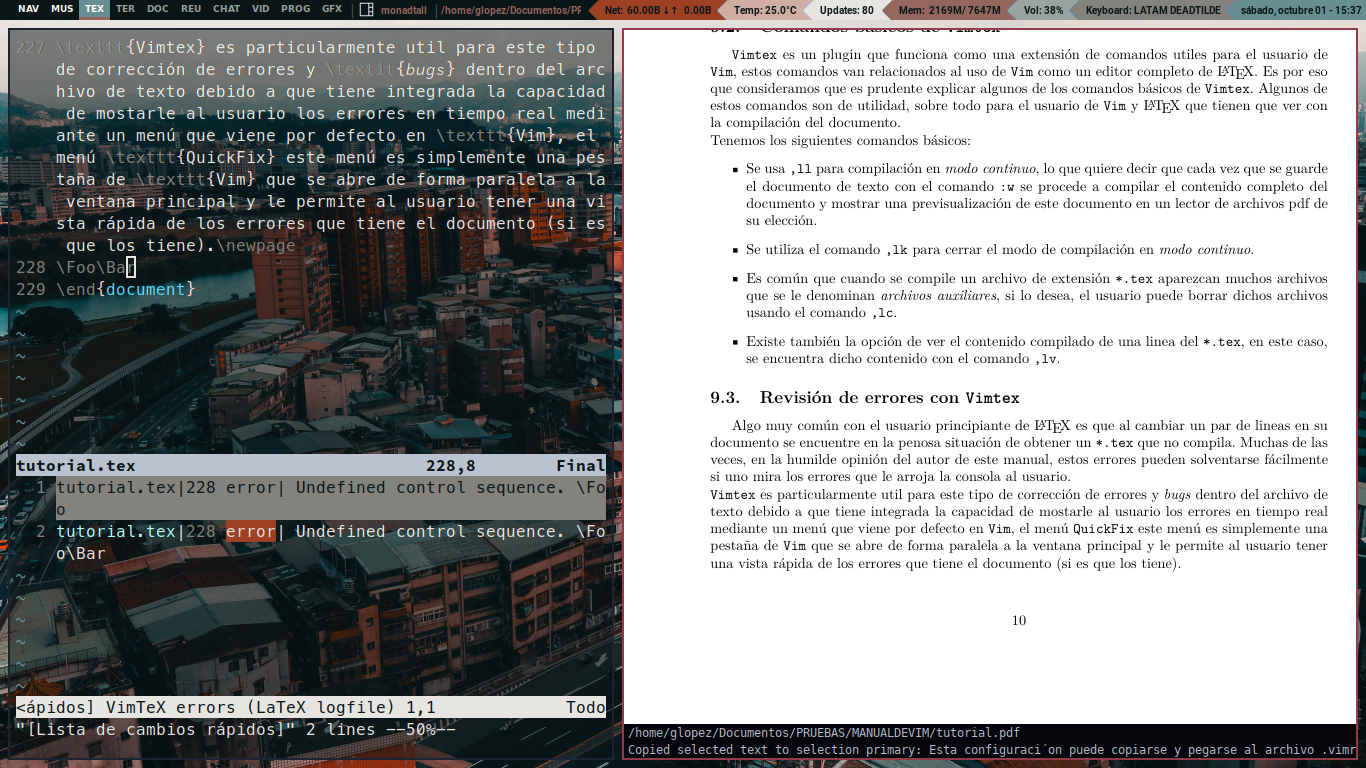
\includegraphics[scale=0.4]{./img/Quickfixmenu.png}
\end{center}
\caption{Vista del menú quickmenu, note que el error de compilación es muy simple. Resulta que los comandos \texttt{Foo} y \texttt{Bar} que se encuentran en la línea 228 del documento no están definidos.}
\label{fig4}
\end{figure}
Puede observar que el menú está en la parte baja de la ventana de \texttt{Vim} y nos comenta que existe un error en la linea 228 del documento \texttt{tutorial.tex} que estamos editando. Además de esto, se nota que en la Figura \ref{fig4}. se observan las bondandes de usar \texttt{Vimtex} para la compilación de estos documentos,se nota que la ventana de la derecha es el documento siendo compilado en tiempo real, lo que le permite al usuario ser más productivo dado que la compilación suele ser un elemento de trabajar en \LaTeX \ que suele tomar su tiempo.\\
Finalmente, le recomendamos al usuario revisar la documentación de \texttt{Vimtex} en su respectivo repositorio de GitHub. Esto con el objetivo de que el lector pueda realizar operaciones mucho más complicadas con este plugin. 
\subsection{¿Es posible moverse entre los diferentes errores de \LaTeX \ en un documento?}
Es normal que un documento de \LaTeX tenga errores en distintas partes del mismo. Por eso, \texttt{Vimtex} agrega al menú \textit{QuickFix} la posibilidad de moverse entre diferentes partes del documento, localizar los errores y corregirlos conforme se vaya necesitando. Para lograr esto, se hace lo siguiente:
\begin{itemize}
	\item Al crearse un error en el documento, se entra al menu \textit{QuickFix} con el comando \texttt{:copen}, esto permite saltar de la venta principal al menú y poder desplazarse en el mismo. 
	\item Presionando la tecla \texttt{Enter} en el error situado dentro del menú \textit{QuickFix} se saltará a la línea que requiera corrección. Esto facilita al usuario revisar si ha escrito algo mal y depurar su archivo más rápido.
	\item Una vez en la linea de destino, cierre la selección del menú \textit{QuickFix} usando el comando \texttt{:cw} de \texttt{Vim}.
	\item Haga la corrección pertinente.
\end{itemize}
Esto se realiza por cada línea que se desea corregir, es interesante observar que cuando se trabaja así, se exige que al trabajar en un \texttt{*.tex} se manejen buenas prácticas de creación de documentos para tener la menor cantidad de errores posibles. Por lo que el usuario se entrena para poder escribir documentos de \LaTeX que contengan pocos errores, lo que mejora sus capacidades de creación. 
\section{Atajos de Teclado para comandos de \LaTeX}
Hasta ahora, tenemos una instalación de \texttt{Vim} que permite hacer dos cosas principales:
\begin{enumerate}
	\item Editar archivos de texto plano. 
	\item Crear, editar y compilar en tiempo real archivos de extensión \texttt{*.tex}. 
\end{enumerate}
Ahora bien, todo esto es bastante sólido en cuento a productividad, pero quizá queremos aumentar la cantidad de trabajo que se desea producir. Una forma de hacer esto es evitar tener que escribir el comando de \LaTeX \ completo. Para ilustrar esto, consideremos el siguiente ejemplo:
\begin{minted}[linenos]{latex}
\begin{figure}
\begin{center}
	\includegraphics[scale=]{Figures/}
\end{center}
\caption{}
\label{fig:}
\end{figure}
\end{minted}
Es evidente pensar que escribir todo esto es particularmente ineficiente, entonces nos preguntamos \textit{¿Existe alguna forma para poder evitar escribir toda la sintaxis del comando?} Resulta que sí, en este caso, existe un plugin de \texttt{Vim} que nos permite usar lo que se conoce en la comunidad como los \textit{snippets}, en este caso, los snippets son atajos de teclado que permiten escribir todo el contenido de un comando o frase usando pocas letras.\\
De nuevo, el plugin para usar los snippets debe instalarse ya sea usando \textbf{Vim-Plug} o de forma manual. El presente manual presenta la siguiente ventaja: si usted colocó la configuración dada en la sección 8 en su \texttt{.vimrc}, ya debería de tener instalado el plugin para poder hacer uso de los snippets. 
Sin embargo, para poder usar los snippets (con el plugin \textit{Ultisnips}) es necesario que su sistema cumpla los siguientes requisitos:
\begin{enumerate}
	\item Su sistema debería de tener una instalación de \texttt{Python3} funcional. 
	\item Su versión de \texttt{Vim} debería de tener la opción de compilado de \texttt{Python} activada. Para saber si su versión tiene esta característica, coloque el siguiente comando dentro de \texttt{Vim}:
	\begin{center}
		\texttt{:echo has("Python3")}
	\end{center}
En el caso de que su versión de \texttt{Vim} sea la adecuada, el comando le debería de arrojar un \texttt{1} como respuesta en la parte inferior de su ventana. 
\end{enumerate}
\newpage
Una vez que tenga todo listo, primero, debe insertar lo siguiente en su \texttt{.vimrc}
\begin{minted}[linenos]{vim}
"La tecla para activar los snippets"
let g:UltiSnipsExpandTrigger       = '<Tab>' 

"Para usar tab y moverse entre snippets "
let g:UltiSnipsJumpForwardTrigger  = '<Tab>'  

"Para usar shift-tab y moverse hacia atrás entre snippets"
let g:UltiSnipsJumpBackwardTrigger = '<S-Tab>'

"Para colocar el directorio de los snippets"
let g:UltiSnipsSnippetDirectories=[$HOME.'/.vim/UltiSnips']
\end{minted}

Para \texttt{Vim}, es común que los snippets se activen con una sola tecla del teclado, en este caso, se recomienda comenzar usando la tecla \texttt{tab} para el uso inicial de los snippets, si luego se desea cambiar el uso de estos, basta con remover la instrucción \texttt{<Tab>} que se ve anteriormente por la tecla de su preferencia. Ya dicho esto, podemos pasar a la parte de configuración de snippets de uso general. 
\subsection{Configuración de Snippets}
Para configurar los Snippets de uso local (para su instalación de Linux) se recomienda primero ir al siguiente directorio. 
\begin{center}
	\url{${HOME}/.vim}
\end{center}
Una vez en el directorio oculto de \texttt{Vim} debe observar que tiene que existir el siguiente árbol de directorios en esta carpeta:
\begin{center}
\begin{forest}
  for tree={
    font=\ttfamily,
    grow'=0,
    child anchor=west,
    parent anchor=south,
    anchor=west,
    calign=first,
    edge path={
      \noexpand\path [draw, \forestoption{edge}]
      (!u.south west) +(7.5pt,0) |- node[fill,inner sep=1.25pt] {} (.child anchor)\forestoption{edge label};
    },
    before typesetting nodes={
      if n=1
        {insert before={[,phantom]}}
        {}
    },
    fit=band,
    before computing xy={l=15pt},
  }
  [\url{${HOME}}
  [\url{.vim}
  [\url{UltiSnips}
  	[\url{tex}]
  ]
  ]
  ]
]
\end{forest}
\end{center}
Si no está alguna de esas carpetas, se le recomienda crearlas usando los comandos de creación de carpetas de Linux. Una vez que tenga este árbol de directorios, deberá crear un archivo en la carpeta \texttt{.tex}, que puede llamar como guste, seguido de la extensión \texttt{.snippets}. Este archivo se utiliza para editar los snippets que el usuario estime convenientes para su flujo de trabajo. Al final debería de tener algo como esto en su arbol de directorios: 
\begin{center}
\begin{forest}
  for tree={
    font=\ttfamily,
    grow'=0,
    child anchor=west,
    parent anchor=south,
    anchor=west,
    calign=first,
    edge path={
      \noexpand\path [draw, \forestoption{edge}]
      (!u.south west) +(7.5pt,0) |- node[fill,inner sep=1.25pt] {} (.child anchor)\forestoption{edge label};
    },
    before typesetting nodes={
      if n=1
        {insert before={[,phantom]}}
        {}
    },
    fit=band,
    before computing xy={l=15pt},
  }
  [\url{${HOME}}
  [\url{.vim}
  [\url{UltiSnips}
  	[\url{tex}
		[\url{archivo.snippets}]
	]
  ]
  ]
  ]
]
\end{forest}	
\end{center}
Con todo esto hecho, solo resta editar (usando \texttt{Vim}) el archivo \texttt{archivo.snippets} de modo que se pueda editar un snippet muy básico y se muestren las capacidades del plugin \textit{UltiSnips}. Dicho esto, se procede a mostrar la estructura básica de un snippet de \texttt{Vim}.
\begin{minted}[linenos]{vim}
snippet {bandera} ["descripción" [opciones]]
{cuerpo snippet}
endsnippet
\end{minted}
Esto puede parecer un poco confuso, por lo que se procede a explicar cuales son los parámetros de importancia.
\begin{itemize}
	\item La \textit{bandera} es la combinación de letras que seguidas de la tecla \texttt{tab}, permite correr el snippet. 
	\item El \textit{cuerpo snippet} es la pieza de codigo\slash frase\slash texto que se quiere escribir mediante el atajo de teclado. 
\end{itemize}
Consideramos conveniente ilustrar esta teoría mediante un ejemplo, por lo que el autor de este manual comparte algunos de los snippets que ha creado para su uso personal:
\begin{minted}[linenos]{vim}
snippet tt "El comando de texto de terminal"
\texttt{$1}$0
endsnippet

snippet ti "El texto en italica"
\textit{$1}$0
endsnippet

snippet tb "El texto en negrita"
\textit{$1}$0
endsnippet

snippet ff "El comando de fraccion"
\frac{$1}{$2}$0
endsnippet

snippet sec "El comando de seccion"
\section{$1}$0
endsnippet

snippet ssec "El comando de subseccion"
\subsection*{$1}$0
endsnippet

snippet env "el comando para entornos"
\begin{$1}
	$2
\end{$1}
$0
endsnippet

snippet fig "El comando para figura"
\begin{figure}
	\centering
	\includegraphics[$1]{$2}
	\caption{$0}
\end{figure}
endsnippet
\end{minted}
El lector ahora quizá se esté preguntando \textit{¿Qué son esos simbolos de dolar seguidos de un número?} En sí, esos símbolos pueden entenderse como la zona en la que se desea que quede el cursor cuando se active el snippet. Es decir, utilizando la tecla \texttt{tab} podemos movernos entre el comando de \LaTeX para colocar los parámetros que queremos editar. Un buen ejemplo es el del snippet con \textit{bandera} \texttt{env}, que visto más de cerca es el siguiente:
\begin{minted}[linenos]{vim}
snippet env "el comando para entornos"
\begin{$1}
	$2
\end{$1}
$0
endsnippet
\end{minted}
En este caso, se nota que el símbolo \texttt{\$1} está presente tanto en el \texttt{begin} como en el \texttt{end} del comando. Esto tiene el siguiente uso: podemos escribir el entorno de \LaTeX que queremos \textit{al mismo tiempo} si configuramos el snippet de la forma que se mostró con anterioridad, por lo que no es necesario escribir el entorno en el \texttt{begin} como en el \texttt{end}, dado que esta configuración permite escribir la frase al mismo tiempo en los dos lugares marcados por el símbolo \texttt{\$1}.
\section{Algunas recomendaciones finales}
Si bien \texttt{Vim} es un editor de texto potente, este tiene una curva de dificultad relativamente pronunciada. Esto no es malo, simplemente se necesita de tiempo para poder acostumbrarse al flujo de trabajo que este software requiere del usuario para poder ser utilizado a su máximo potencial. \\
Se recomienda antes de realizar todo el trabajo de configuración visto en este manual, primero, revisar el complemento \texttt{vimtutor} para poder tener cierta soltura con los comandos básicos de \texttt{Vim} y la navegación básica que este software ofrece. Además de esto, si bien es cierto que este manual va orientado a integrar \texttt{Vim} con \LaTeX, es necesario recalcar que en realidad, \texttt{Vim} es una herramienta de uso general y puede configurarse para usarse como \textit{IDE} de cualquier plataforma de programación, por lo que es de principal utilidad a aquellos desarrolladores que desean un \textit{IDE} minimalista y veloz. Por lo comentado anteriormente, el autor de este manual exhorta al lector a revisar otros usos de \texttt{Vim} orientados más bien al desarrollo software. 
\end{document}
